\chapter{Internet of Things}

\section{Inside IoT}
\subsection{Hardware components}
IoT devices contain \textbf{sensors}, \textbf{actuators}, or \textit{both}.
\begin{itemize}
   \item \textbf{Sensors} $\longrightarrow$ \textit{acquire data}\\
   Monitor Things and provide data about the Thing, like temperature, light intensity, or battery level.
   \item \textbf{Actuators} $\longrightarrow$ \textit{control/act on data}\\
   Control Things through hardware in the device;
   they represent the physical
   interface to the Thing that "make it go"
   \note{
      e.g. controls in a smart thermostat, dimmer switch in a smart light bulb, or motors in a robotic vacuum cleaner.
   }
\end{itemize}

All IoT devices have a way to process sensor data, store {--}if necessary{--} such data locally, and provide the computing power that makes the device
operate.
The data \textbf{processing component} of the IoT device coordinates data from multiple sensors or stores in flash memory.

\subsection{Firmware}
The \textbf{Firmware} is the onboard software that runs an IoT device sits between the
hardware and the outside world.

For simpler resource-constrained devices the firmware may be \textbf{embedded}.
More advanced devises instead nowdays have an entire \textbf{OS} as firmware, providing an
\textit{abstraction layer} between the hardware and other software on the device.
\note{A popular OS choice is \href{https://busybox.net/}{\textbf{Busybox}}}

\section{IoT Attacks}
\textbf{Security} is usually an \textit{\underline{afterthought}} in IoT because it is difficult to create a cheap reliable, resource-constrained device that can connect to a wireless network, having very little power consumption.

\labelitemize{Attack Vectors}{
\begin{enumerate}
   \item \textbf{Weak Passwords}\\
   To simplify the device setup and use, the manufacturer offers typically weak login credentials
   \item \textbf{Lack of encryption}\\
   Many IoT devices do \textit{not} support encryption,
   to save battery and performance.
   \item \textbf{Backdoor}\\
   Is common practice for manufacturers to put "hidden" access mechanisms to simplify the support. 
   Once a backdoor becomes known, the manufacturer can either remove it, or make it more difficult to be accessed (or so they think \smiley)
   \item \textbf{Internet Exposure}\\
   Unlike a hardened server where you can control the firewall and how the host is accessed, most IoT
   devices have little or no security and accept most internet traffic, 
   making them susceptible to attack.
\end{enumerate}
}
\labelitemize{Countermeasures}{
   \begin{enumerate}
      \item Always \textbf{change} the \textit{default password}
      \item \textbf{Remove} devices with \textit{telnet backdoors}
      \begin{enumerate}
         \item To discover such devices you can use IoT device scanners that
         check with \href{https://www.shodan.io/}{\textbf{Shodan}}, an IoT search engine, to reveal if your devices
         are vulnerable based on the IP address of the scanning computer.
      \end{enumerate}
      \item \textbf{Never expose} a device directly to the internet
      \begin{enumerate}
         \item When you consider whether or not to expose a device to the
         internet by opening up your firewall, the right answer is almost
         \textbf{always no}.
      \end{enumerate}
      \item IoT device scanner can run a \textit{"deep scan"} to check for any open
      ports on your publicly exposed IP address assigned by your ISP.
      \begin{enumerate}
         \item \textbf{Port Scan} all your machines
      \end{enumerate}
   \end{enumerate}
}

\subsection{Shodan}
\href{https://www.shodan.io/}{\textbf{Shodan}} is a \textit{search engine} for finding specific devices, and
device types, that exist online.\\
The most popular searches are for things like webcam, linksys, cisco, netgear, SCADA, Default password.

It uses a specialized scanner to \underline{scan the \textbf{entire Internet}} and parse the banners that are returned by various devices.
\note{
   Shodan can tell things like what web server {--}and
   version{--} is most popular, or how many anonymous FTP
   servers exist in a particular location, and what make and
   model the device may be.
}
You start by navigating to the main page, and then entering
into the search field, like you would any other search engine.

\begin{figure}[htbp]
   \centering
   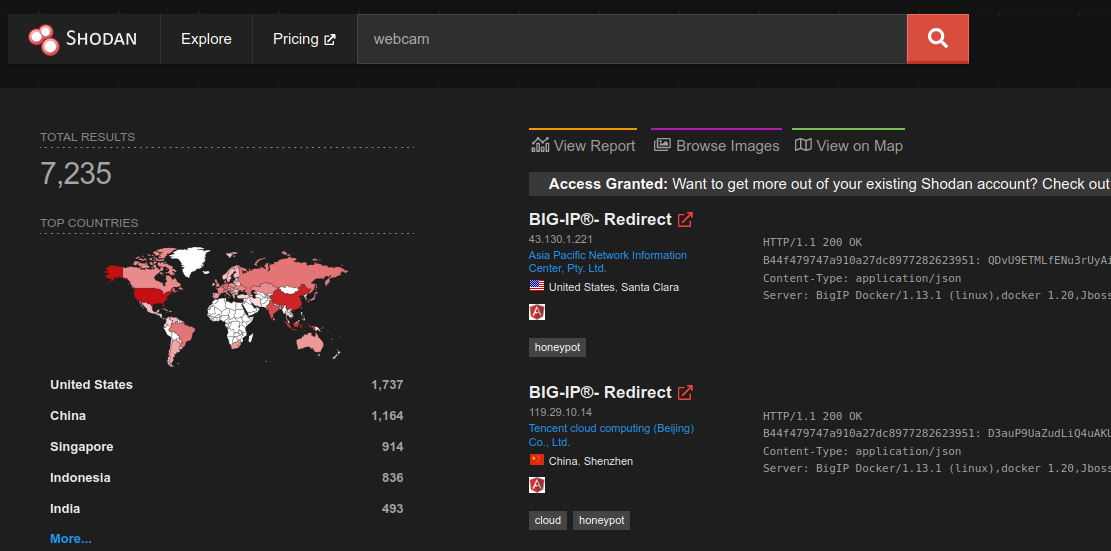
\includegraphics{images/shodan.png}
   \caption{Shodan search screenshot}
   \label{fig:shodan}
\end{figure}

\section{Device Classification}
IoT Nodes may be classified by performance or functionally
\labelitemize{Performance}{
\begin{enumerate}
   \item \textbf{Ultra-constrained} node\\
   RTOS or bare metal with 16K of RAM.
   Energy harvesting limits radio transmissions to conserve power.
   \item \textbf{Constrained} node\\
   RTOS with 32K-64K RAM.
   Most likely running on a battery and software optimised for battery life.
   Again minimizing radio transmission
   \item \textbf{Mainstream} node\\
   A feature rich RTOS with 128K RAM.
   More complex interaction with the context since there is room for more local operation, as opposed to sending all data upstream.
   \item \textbf{Gateway} node\\
   An advanced OS with 64MB RAM.
   A sophisticated node with advanced software and runs from main power.
   Multiple radios to support the local network.
\end{enumerate}
}

\labelitemize{Functional}{
\begin{enumerate}
   \item \textbf{Simple node}\\
   Not aware of the rest of the local network.
   It collects and
   reports information to the specified destination.
   Any of previous 1-3
   may be a simple node it depends upon interactions.
   \item \textbf{Smart node}\\
   fully aware of all other network nodes mainly via software
   that understands mesh networks, local topologies and authorised
   interactions between nodes in the same network.
   \item \textbf{Access node}\\
   the edge box to connect the local network to the Internet
   via whatever broadband link is appropriate for the application.
   It has
   multiple radios facing the local network.
   \item No restrictions on creating a node that is a smart node and acts as a
   gateway.
\end{enumerate}
}